{\color{PineGreen}\section{Summary}}

This document is a report written during the \textbf{Hack the Crisis NL} online hacakthon\cite{bib1}. We propose a system for secure and privacy-preserving contact tracing. Providing a technological foundation to help slow the spread of the SARS-CoV-2 virus.\\

Goals:
\begin{itemize}
\item Take advantage of existing implemented solutions to brake transmission chains and control the spread of the disease,
\item Avoid Identity Driven solutions. We don't ask citizens to provide their identity,
\item Inform the user if there is an infection in their contact chain,
\item Automate the process of inferring the list of possible users that might have been exposed to an infected person in the 14 days preceding the test
\end{itemize} 

The system aims to minimise single point of failure, privacy and security risks for citizens and communities and to guarantee data protection.

To achieve this goal, we use mobile applications to continuously track anonymous users (we do not ask them to provide email,name, surname or ID numbers) and ask them to report symptoms, if they are using Individual Protection Devices or protective clothing when they go out. The information is encrypted and stored in an ummutable decentralized digital ledger called Tangle. 
Whenever a patient is diagnosed, verified Health Departments, testing laboratories or Drive In testing facilities send his universal unique identifier (uuid) of the the application to the Tangle and flags it as an infected uuid. \\
\\
As soon as a new infected uuid is published on the ledger a computer (no server is required, works with a personal computer as well) performs the contact tracing task and uuids at risk are broadcasted.\\
If the application sees its uuid on the Tangle, the user is notified of the risk so that he/she can then take preventive actions such as self-isolating or wearing a ffp3 mask.

\begin{figure}[H]
	\begin{center}
	    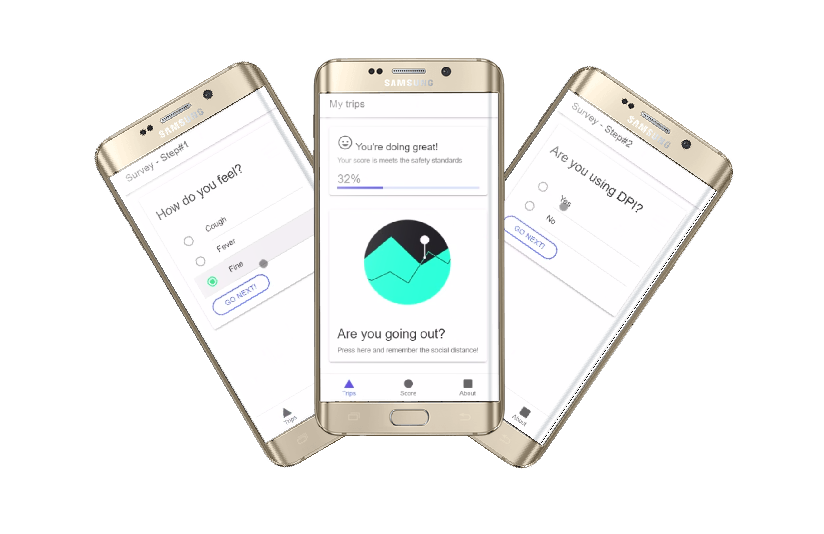
\includegraphics[scale=0.9]{imgs/phones_1.pdf}
 		\caption{Self-report information about the symptoms}
 		\label{fig:hi_low}
	\end{center}
\end{figure}


%pseudo-random ID representing the user and also record pseudo-random IDs observed from
%smartphones in close proximity. Whenever a patient is diagnosed, he or she can upload
%some anonymous data from their phone to a central server. This step should only be done
%with the approval of a health authority and the consent of the individual. Before, no data is
%communicated to any entity. Other instances of the app can use the anonymous data from
%the server to locally compute whether the app's user was in physical proximity and
%potentially infected by an infected person and to inform the user of the risk. Additionally, the
%system enables users to voluntarily provide information to epidemiologists, in a
%privacy-preserving manner, to enable studies of the evolution of disease and to assist in
%finding better policies to prevent further infections

The architecture of the system is depicted below:
\begin{figure}[H]
	\begin{center}
	    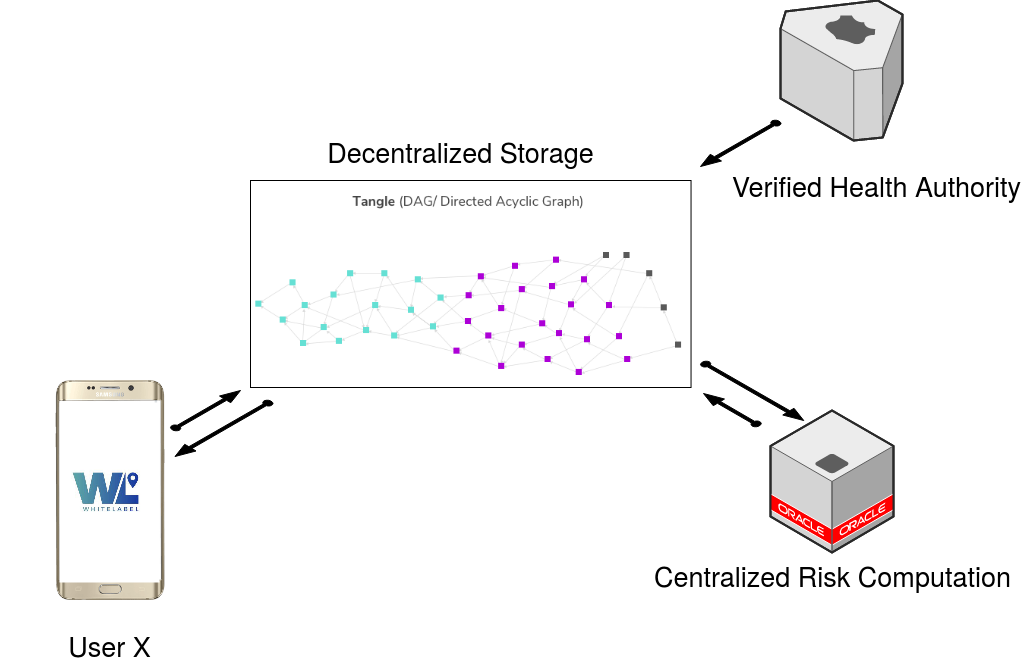
\includegraphics[scale=0.3]{imgs/arch.png}
 		\caption{}
 		\label{fig:hi_low}
	\end{center}
\end{figure}

Additionally, the system enables users to voluntarily provide information to epidemiologists to enable studies of the evolution of disease in the region of interest and to assist in finding better policies to prevent further infections.\\

The code is available on Github and released under the GNU GPL v3 license so that further protection mechanisms can be added if weaknesses are identified and additional features can be added by the community.
%
%\begin{equation}
%    \chi = \begin{bmatrix}
%        x \\ y \\ \theta
%     \end{bmatrix}\qquad \qquad
%Y = \begin{bmatrix}
%        y \\ \theta
%     \end{bmatrix}\qquad \qquad
%U = \omega
%\end{equation}
%in which:
%\begin{itemize}
%	\item x, y: Linear positions of the center of the camera respectively along the x and y axes
%	\item $\theta$: Angular position of the center of the camera along the z-axis
%	\item $\omega$: Angular velocity along the z-axis which represents the input of the system
%	\item v: velocity vector of the center of gravity of the robot. Assumed to be constant
%\end{itemize}
%The following subsections present dynamic models considered in during the simulation and design of the controller
%{\color{PineGreen}\subsection{Simplified system}}
%Discrete system with sampling time $\delta_{T}$
%\begin{align}
%    x(k+1) ={} & x(k) + \vert v \vert \delta_{T} cos(\theta(k))
%\\
%	y(k+1) ={} & y(k) + \vert v \vert \delta_{T} sin(\theta(k))\label{eq:pointMass}
%\\
%	\theta(k+1) = {} &  \theta(k)+\omega(k) \delta_{T} =  \theta(k)+u(k) \delta_{T} 
%\end{align}
%
%{\color{PineGreen}\subsection{Perturbed Simplified system}}
%In a real world scenario, Toutilo's description can be affected by unmodeled dynamics which force the robot to steer towards an unknown direction even if no angular velocity command is executed. This phenomenon can be approximated by an uncertain constant angular velocity drift $\omega_{D}$. In addition, when driving over low-traction, deformable terrains or even steep hills, external forces have to be considered in order to achieve acceptable results. An approximation of these forces can be introduced in the system by considering a linear velocity component $v_{y}$.
%\\
%\begin{itemize}
%	\item $\omega_{D}$ : Angular drift along the z-axis. [ Uncertainty ]
%	\item $v_{y}$ : linear velocity vector resulting from an external force acting on the center of mass of the robotic platform [ external forces ]
%\end{itemize}
%
%The resulting discrete system is described by:
%\begin{equation}
%    x(k+1) = x(k) + [\vert v \vert  cos(\theta(k)) - \vert v_{y} \vert sin(\theta(k))]\delta_{T}
%\end{equation}
%\begin{equation}
%    y(k+1) = y(k) + [\vert v \vert  sin(\theta(k)) + \vert v_{y} \vert cos(\theta(k))]\delta_{T}
%\end{equation}	
%\begin{equation}
%   	\theta(k+1) = \theta(k)+(u(k)+\omega_D) \delta_{T} 
%\end{equation}
%
%{\color{PineGreen}\subsection{Perturbed and constrained Simplified system}\label{subsec:pertconstrained}}
%
%It is worth noting that the low level controller of Toutilo presents several non-linearities that have to be taken into account during the design of the control system. A dead zone of $ \pm 5 mrad/s$ associated to the control input $\omega$.\newline
%\\
%Let us introduce two new inputs:
%\begin{itemize}
%	\item $u_S = sat(u(\cdot), max, min)$ : is a saturation function of the control input
%	\item $u_D = deadZ(u(\cdot), max, min)$ : is a dead zone applied to the control input
%\end{itemize}
%The new system is described by:
%\begin{equation}
%    x(k+1) = x(k) + [\vert v \vert  cos(\theta(k)) - \vert v_{y} \vert sin(\theta(k))]\delta_{T}
%\end{equation}
%\begin{equation}
%    y(k+1) = y(k) + [\vert v \vert  sin(\theta(k)) + \vert v_{y} \vert cos(\theta(k))]\delta_{T}
%\end{equation}	
%\begin{equation}
%   	\theta(k+1) = \theta(k)+(u_S(k)+\omega_D) \delta_{T} 
%\end{equation}
%\begin{equation}
%   	u_S = sat(u_D(k), max_{sat}, min_{sat})
%\end{equation}
%\begin{equation}
%   	u_D = deadZ(u(k), max_{deadZ}, min_{deadZ})
%\end{equation}
%
%{\color{PineGreen}\subsection{Differential Drive system}}
%
%
%{\color{PineGreen}\subsection{Perturbed and constrained Differential Drive system}}